% Options for packages loaded elsewhere
\PassOptionsToPackage{unicode}{hyperref}
\PassOptionsToPackage{hyphens}{url}
\PassOptionsToPackage{dvipsnames,svgnames,x11names}{xcolor}
%
\documentclass[
  letterpaper,
  DIV=11,
  numbers=noendperiod]{scrartcl}

\usepackage{amsmath,amssymb}
\usepackage{iftex}
\ifPDFTeX
  \usepackage[T1]{fontenc}
  \usepackage[utf8]{inputenc}
  \usepackage{textcomp} % provide euro and other symbols
\else % if luatex or xetex
  \usepackage{unicode-math}
  \defaultfontfeatures{Scale=MatchLowercase}
  \defaultfontfeatures[\rmfamily]{Ligatures=TeX,Scale=1}
\fi
\usepackage{lmodern}
\ifPDFTeX\else  
    % xetex/luatex font selection
\fi
% Use upquote if available, for straight quotes in verbatim environments
\IfFileExists{upquote.sty}{\usepackage{upquote}}{}
\IfFileExists{microtype.sty}{% use microtype if available
  \usepackage[]{microtype}
  \UseMicrotypeSet[protrusion]{basicmath} % disable protrusion for tt fonts
}{}
\makeatletter
\@ifundefined{KOMAClassName}{% if non-KOMA class
  \IfFileExists{parskip.sty}{%
    \usepackage{parskip}
  }{% else
    \setlength{\parindent}{0pt}
    \setlength{\parskip}{6pt plus 2pt minus 1pt}}
}{% if KOMA class
  \KOMAoptions{parskip=half}}
\makeatother
\usepackage{xcolor}
\setlength{\emergencystretch}{3em} % prevent overfull lines
\setcounter{secnumdepth}{-\maxdimen} % remove section numbering
% Make \paragraph and \subparagraph free-standing
\ifx\paragraph\undefined\else
  \let\oldparagraph\paragraph
  \renewcommand{\paragraph}[1]{\oldparagraph{#1}\mbox{}}
\fi
\ifx\subparagraph\undefined\else
  \let\oldsubparagraph\subparagraph
  \renewcommand{\subparagraph}[1]{\oldsubparagraph{#1}\mbox{}}
\fi

\usepackage{color}
\usepackage{fancyvrb}
\newcommand{\VerbBar}{|}
\newcommand{\VERB}{\Verb[commandchars=\\\{\}]}
\DefineVerbatimEnvironment{Highlighting}{Verbatim}{commandchars=\\\{\}}
% Add ',fontsize=\small' for more characters per line
\usepackage{framed}
\definecolor{shadecolor}{RGB}{241,243,245}
\newenvironment{Shaded}{\begin{snugshade}}{\end{snugshade}}
\newcommand{\AlertTok}[1]{\textcolor[rgb]{0.68,0.00,0.00}{#1}}
\newcommand{\AnnotationTok}[1]{\textcolor[rgb]{0.37,0.37,0.37}{#1}}
\newcommand{\AttributeTok}[1]{\textcolor[rgb]{0.40,0.45,0.13}{#1}}
\newcommand{\BaseNTok}[1]{\textcolor[rgb]{0.68,0.00,0.00}{#1}}
\newcommand{\BuiltInTok}[1]{\textcolor[rgb]{0.00,0.23,0.31}{#1}}
\newcommand{\CharTok}[1]{\textcolor[rgb]{0.13,0.47,0.30}{#1}}
\newcommand{\CommentTok}[1]{\textcolor[rgb]{0.37,0.37,0.37}{#1}}
\newcommand{\CommentVarTok}[1]{\textcolor[rgb]{0.37,0.37,0.37}{\textit{#1}}}
\newcommand{\ConstantTok}[1]{\textcolor[rgb]{0.56,0.35,0.01}{#1}}
\newcommand{\ControlFlowTok}[1]{\textcolor[rgb]{0.00,0.23,0.31}{#1}}
\newcommand{\DataTypeTok}[1]{\textcolor[rgb]{0.68,0.00,0.00}{#1}}
\newcommand{\DecValTok}[1]{\textcolor[rgb]{0.68,0.00,0.00}{#1}}
\newcommand{\DocumentationTok}[1]{\textcolor[rgb]{0.37,0.37,0.37}{\textit{#1}}}
\newcommand{\ErrorTok}[1]{\textcolor[rgb]{0.68,0.00,0.00}{#1}}
\newcommand{\ExtensionTok}[1]{\textcolor[rgb]{0.00,0.23,0.31}{#1}}
\newcommand{\FloatTok}[1]{\textcolor[rgb]{0.68,0.00,0.00}{#1}}
\newcommand{\FunctionTok}[1]{\textcolor[rgb]{0.28,0.35,0.67}{#1}}
\newcommand{\ImportTok}[1]{\textcolor[rgb]{0.00,0.46,0.62}{#1}}
\newcommand{\InformationTok}[1]{\textcolor[rgb]{0.37,0.37,0.37}{#1}}
\newcommand{\KeywordTok}[1]{\textcolor[rgb]{0.00,0.23,0.31}{#1}}
\newcommand{\NormalTok}[1]{\textcolor[rgb]{0.00,0.23,0.31}{#1}}
\newcommand{\OperatorTok}[1]{\textcolor[rgb]{0.37,0.37,0.37}{#1}}
\newcommand{\OtherTok}[1]{\textcolor[rgb]{0.00,0.23,0.31}{#1}}
\newcommand{\PreprocessorTok}[1]{\textcolor[rgb]{0.68,0.00,0.00}{#1}}
\newcommand{\RegionMarkerTok}[1]{\textcolor[rgb]{0.00,0.23,0.31}{#1}}
\newcommand{\SpecialCharTok}[1]{\textcolor[rgb]{0.37,0.37,0.37}{#1}}
\newcommand{\SpecialStringTok}[1]{\textcolor[rgb]{0.13,0.47,0.30}{#1}}
\newcommand{\StringTok}[1]{\textcolor[rgb]{0.13,0.47,0.30}{#1}}
\newcommand{\VariableTok}[1]{\textcolor[rgb]{0.07,0.07,0.07}{#1}}
\newcommand{\VerbatimStringTok}[1]{\textcolor[rgb]{0.13,0.47,0.30}{#1}}
\newcommand{\WarningTok}[1]{\textcolor[rgb]{0.37,0.37,0.37}{\textit{#1}}}

\providecommand{\tightlist}{%
  \setlength{\itemsep}{0pt}\setlength{\parskip}{0pt}}\usepackage{longtable,booktabs,array}
\usepackage{calc} % for calculating minipage widths
% Correct order of tables after \paragraph or \subparagraph
\usepackage{etoolbox}
\makeatletter
\patchcmd\longtable{\par}{\if@noskipsec\mbox{}\fi\par}{}{}
\makeatother
% Allow footnotes in longtable head/foot
\IfFileExists{footnotehyper.sty}{\usepackage{footnotehyper}}{\usepackage{footnote}}
\makesavenoteenv{longtable}
\usepackage{graphicx}
\makeatletter
\def\maxwidth{\ifdim\Gin@nat@width>\linewidth\linewidth\else\Gin@nat@width\fi}
\def\maxheight{\ifdim\Gin@nat@height>\textheight\textheight\else\Gin@nat@height\fi}
\makeatother
% Scale images if necessary, so that they will not overflow the page
% margins by default, and it is still possible to overwrite the defaults
% using explicit options in \includegraphics[width, height, ...]{}
\setkeys{Gin}{width=\maxwidth,height=\maxheight,keepaspectratio}
% Set default figure placement to htbp
\makeatletter
\def\fps@figure{htbp}
\makeatother

\KOMAoption{captions}{tableheading}
\makeatletter
\@ifpackageloaded{caption}{}{\usepackage{caption}}
\AtBeginDocument{%
\ifdefined\contentsname
  \renewcommand*\contentsname{Table of contents}
\else
  \newcommand\contentsname{Table of contents}
\fi
\ifdefined\listfigurename
  \renewcommand*\listfigurename{List of Figures}
\else
  \newcommand\listfigurename{List of Figures}
\fi
\ifdefined\listtablename
  \renewcommand*\listtablename{List of Tables}
\else
  \newcommand\listtablename{List of Tables}
\fi
\ifdefined\figurename
  \renewcommand*\figurename{Figure}
\else
  \newcommand\figurename{Figure}
\fi
\ifdefined\tablename
  \renewcommand*\tablename{Table}
\else
  \newcommand\tablename{Table}
\fi
}
\@ifpackageloaded{float}{}{\usepackage{float}}
\floatstyle{ruled}
\@ifundefined{c@chapter}{\newfloat{codelisting}{h}{lop}}{\newfloat{codelisting}{h}{lop}[chapter]}
\floatname{codelisting}{Listing}
\newcommand*\listoflistings{\listof{codelisting}{List of Listings}}
\makeatother
\makeatletter
\makeatother
\makeatletter
\@ifpackageloaded{caption}{}{\usepackage{caption}}
\@ifpackageloaded{subcaption}{}{\usepackage{subcaption}}
\makeatother
\ifLuaTeX
  \usepackage{selnolig}  % disable illegal ligatures
\fi
\usepackage{bookmark}

\IfFileExists{xurl.sty}{\usepackage{xurl}}{} % add URL line breaks if available
\urlstyle{same} % disable monospaced font for URLs
\hypersetup{
  pdftitle={Exploartion\_17 : Tree-Based Genetic Programming for Polynomial Regression},
  pdfauthor={Mohammed Tawheed Khater},
  colorlinks=true,
  linkcolor={blue},
  filecolor={Maroon},
  citecolor={Blue},
  urlcolor={Blue},
  pdfcreator={LaTeX via pandoc}}

\title{Exploartion\_17 : Tree-Based Genetic Programming for Polynomial
Regression}
\usepackage{etoolbox}
\makeatletter
\providecommand{\subtitle}[1]{% add subtitle to \maketitle
  \apptocmd{\@title}{\par {\large #1 \par}}{}{}
}
\makeatother
\subtitle{this is for
\texttt{matlab\_translation\_symbolic\_regression\_18.m} file
implementation}
\author{Mohammed Tawheed Khater}
\date{2024-06-23}

\begin{document}
\maketitle
\begin{abstract}
This document is intended to be a simpler alternative for translating
symbolic regression code from Python to MATLAB. It focuses on a more
straightforward approach, as translating the Node and Tree classes from
the Python code on GitHub
\href{https://github.com/dyckia/Genetic-Programming-Polynomial-Regression}{(by
dyckia, titled ``Genetic-Programming-Polynomial-Regression'')} proved
challenging.

a complete example working matlab file
\texttt{matlab\_translation\_symbolic\_regression\_18.m} will be sent
with this document via whatsapp.

later i will upload it to github with proper permenant link.

here is link the translated file : -
\href{https://github.com/MohammedTwheed/dr-farid-genetic-programming-polynomial-regression-convert-to-matlab/blob/master/2024-06-22/SymboicRegression_02/matlab_translation_symbolic_regression_18.m}{matlab\_translation\_symbolic\_regression\_18.m}

here is link to the training data used : -
\href{https://github.com/MohammedTwheed/dr-farid-genetic-programming-polynomial-regression-convert-to-matlab/blob/master/A4_trainingSamples.txt}{A4\_trainingSamples.txt}
\end{abstract}

\renewcommand*\contentsname{Table of Contents}
{
\hypersetup{linkcolor=}
\setcounter{tocdepth}{3}
\tableofcontents
}
\subsection{download this doc as pdf or
word}\label{download-this-doc-as-pdf-or-word}

Other Formats

PDF

MS Word

\subsection{Introduction}\label{introduction}

Symbolic regression, a technique used to identify mathematical
expressions that best fit a given dataset, is a complex task often
tackled using genetic programming (GP). Genetic programming mimics
natural evolution to optimize candidate solutions, represented as
mathematical expressions. This review explores the implementation of a
genetic algorithm for symbolic regression using MATLAB, delving into the
detailed structure of the genetic algorithm and the representation of
mathematical expressions as tree structures. The following sections will
elaborate on the genetic algorithm's key components, the tree structure
for representing mathematical expressions, and the nuances of the MATLAB
implementation.

\subsection{Genetic Algorithm
Implementation}\label{genetic-algorithm-implementation}

The genetic algorithm (GA) for symbolic regression involves several
critical steps: population initialization, selection, crossover,
mutation, and fitness evaluation. Each of these steps is meticulously
implemented in MATLAB to evolve mathematical expressions that best fit
the provided data.

\subsubsection{1. Population
Initialization}\label{population-initialization}

Population initialization is achieved using the ramped half-and-half
method, which ensures a diverse initial population. This method
generates trees with varying depths and structures, promoting genetic
diversity.

\begin{Shaded}
\begin{Highlighting}[]
\KeywordTok{function} \VariableTok{pop} \OperatorTok{=} \VariableTok{initialPopulation}\NormalTok{(}\VariableTok{pop\_size}\OperatorTok{,} \VariableTok{max\_depth}\OperatorTok{,} \VariableTok{terminal\_set}\OperatorTok{,} \VariableTok{function\_set}\NormalTok{)}
    \VariableTok{pop} \OperatorTok{=} \VariableTok{cell}\NormalTok{(}\FloatTok{1}\OperatorTok{,} \VariableTok{pop\_size}\NormalTok{)}\OperatorTok{;}
    \KeywordTok{for} \VariableTok{i} \OperatorTok{=} \FloatTok{1}\OperatorTok{:}\VariableTok{pop\_size}
        \VariableTok{method} \OperatorTok{=} \SpecialStringTok{\textquotesingle{}full\textquotesingle{}}\OperatorTok{;}
        \KeywordTok{if} \VariableTok{i} \OperatorTok{\textgreater{}}\NormalTok{ (}\VariableTok{pop\_size} \OperatorTok{/} \FloatTok{2}\NormalTok{)}
            \VariableTok{method} \OperatorTok{=} \SpecialStringTok{\textquotesingle{}grow\textquotesingle{}}\OperatorTok{;}
        \KeywordTok{end}
        \VariableTok{pop}\NormalTok{\{}\VariableTok{i}\NormalTok{\} }\OperatorTok{=} \VariableTok{growTree}\NormalTok{(}\VariableTok{max\_depth}\OperatorTok{,} \VariableTok{method}\OperatorTok{,} \FloatTok{0}\OperatorTok{,} \VariableTok{terminal\_set}\OperatorTok{,} \VariableTok{function\_set}\NormalTok{)}\OperatorTok{;}
    \KeywordTok{end}
    \VariableTok{pop} \OperatorTok{=} \VariableTok{pop}\NormalTok{(}\VariableTok{randperm}\NormalTok{(}\VariableTok{length}\NormalTok{(}\VariableTok{pop}\NormalTok{)))}\OperatorTok{;}  \CommentTok{\% Randomize the population}
\KeywordTok{end}
\end{Highlighting}
\end{Shaded}

The \texttt{growTree} function generates individual trees using either
the ``full'' method, creating fully populated trees to the maximum
depth, or the ``grow'' method, generating trees with random depths.

\subsubsection{2. Selection}\label{selection}

Tournament selection is employed to choose individuals for reproduction.
This method ensures that individuals with better fitness are more likely
to be selected, driving the population towards better solutions.

\begin{Shaded}
\begin{Highlighting}[]
\KeywordTok{function} \VariableTok{selected} \OperatorTok{=} \VariableTok{tournamentSelection}\NormalTok{(}\VariableTok{pop}\OperatorTok{,} \VariableTok{tour\_size}\OperatorTok{,} \VariableTok{x}\OperatorTok{,} \VariableTok{y}\OperatorTok{,} \VariableTok{rf}\OperatorTok{,} \VariableTok{terminal\_set}\NormalTok{)}
    \VariableTok{selected\_ind} \OperatorTok{=} \VariableTok{randperm}\NormalTok{(}\VariableTok{length}\NormalTok{(}\VariableTok{pop}\NormalTok{)}\OperatorTok{,} \VariableTok{tour\_size}\NormalTok{)}\OperatorTok{;}
    \VariableTok{selected} \OperatorTok{=} \VariableTok{cell}\NormalTok{(}\VariableTok{tour\_size}\OperatorTok{,} \FloatTok{2}\NormalTok{)}\OperatorTok{;}
    \KeywordTok{for} \VariableTok{i} \OperatorTok{=} \FloatTok{1}\OperatorTok{:}\VariableTok{tour\_size}
        \VariableTok{tree} \OperatorTok{=} \VariableTok{pop}\NormalTok{\{}\VariableTok{selected\_ind}\NormalTok{(}\VariableTok{i}\NormalTok{)\}}\OperatorTok{;}
        \VariableTok{fitness} \OperatorTok{=} \VariableTok{computeError}\NormalTok{(}\VariableTok{tree}\OperatorTok{,} \VariableTok{x}\OperatorTok{,} \VariableTok{y}\OperatorTok{,} \VariableTok{rf}\OperatorTok{,} \VariableTok{terminal\_set}\NormalTok{)}\OperatorTok{;}
        \VariableTok{selected}\NormalTok{\{}\VariableTok{i}\OperatorTok{,} \FloatTok{1}\NormalTok{\} }\OperatorTok{=} \VariableTok{tree}\OperatorTok{;}
        \VariableTok{selected}\NormalTok{\{}\VariableTok{i}\OperatorTok{,} \FloatTok{2}\NormalTok{\} }\OperatorTok{=} \VariableTok{fitness}\OperatorTok{;}
    \KeywordTok{end}
    \VariableTok{selected} \OperatorTok{=} \VariableTok{sortrows}\NormalTok{(}\VariableTok{selected}\OperatorTok{,} \FloatTok{2}\NormalTok{)}\OperatorTok{;}  \CommentTok{\% Sort based on fitness (ascending)}
\KeywordTok{end}
\end{Highlighting}
\end{Shaded}

Tournament selection enhances the likelihood of selecting fitter
individuals while maintaining some level of genetic diversity, which is
crucial for avoiding local optima.

\subsubsection{3. Crossover}\label{crossover}

Crossover involves exchanging subtrees between pairs of parent trees to
produce offspring with mixed characteristics. This operation introduces
variability and combines the strengths of both parents.

\begin{Shaded}
\begin{Highlighting}[]
\KeywordTok{function}\NormalTok{ [}\VariableTok{tree1}\OperatorTok{,} \VariableTok{tree2}\NormalTok{] }\OperatorTok{=} \VariableTok{crossover}\NormalTok{(}\VariableTok{tree1}\OperatorTok{,} \VariableTok{tree2}\OperatorTok{,} \VariableTok{c\_rate}\NormalTok{)}
    \KeywordTok{if} \VariableTok{rand}\NormalTok{() }\OperatorTok{\textless{}=} \VariableTok{c\_rate}
        \VariableTok{swap\_point1} \OperatorTok{=} \VariableTok{randi}\NormalTok{([}\FloatTok{0}\OperatorTok{,} \VariableTok{countNodes}\NormalTok{(}\VariableTok{tree1}\NormalTok{) }\OperatorTok{{-}} \FloatTok{1}\NormalTok{])}\OperatorTok{;}
        \VariableTok{swap\_point2} \OperatorTok{=} \VariableTok{randi}\NormalTok{([}\FloatTok{0}\OperatorTok{,} \VariableTok{countNodes}\NormalTok{(}\VariableTok{tree2}\NormalTok{) }\OperatorTok{{-}} \FloatTok{1}\NormalTok{])}\OperatorTok{;}
        \VariableTok{subtree1} \OperatorTok{=} \VariableTok{getSubtree}\NormalTok{(}\VariableTok{tree1}\OperatorTok{,} \VariableTok{swap\_point1}\NormalTok{)}\OperatorTok{;}
        \VariableTok{subtree2} \OperatorTok{=} \VariableTok{getSubtree}\NormalTok{(}\VariableTok{tree2}\OperatorTok{,} \VariableTok{swap\_point2}\NormalTok{)}\OperatorTok{;}
        \VariableTok{tree1} \OperatorTok{=} \VariableTok{setSubtree}\NormalTok{(}\VariableTok{tree1}\OperatorTok{,} \VariableTok{swap\_point1}\OperatorTok{,} \VariableTok{subtree2}\NormalTok{)}\OperatorTok{;}
        \VariableTok{tree2} \OperatorTok{=} \VariableTok{setSubtree}\NormalTok{(}\VariableTok{tree2}\OperatorTok{,} \VariableTok{swap\_point2}\OperatorTok{,} \VariableTok{subtree1}\NormalTok{)}\OperatorTok{;}
    \KeywordTok{end}
\KeywordTok{end}
\end{Highlighting}
\end{Shaded}

\subsubsection{4. Mutation}\label{mutation}

Mutation introduces random changes in the tree structure, which is
essential for maintaining genetic diversity and exploring new solutions.

\begin{Shaded}
\begin{Highlighting}[]
\KeywordTok{function} \VariableTok{tree} \OperatorTok{=} \VariableTok{mutate}\NormalTok{(}\VariableTok{tree}\OperatorTok{,} \VariableTok{m\_rate}\OperatorTok{,} \VariableTok{max\_depth}\OperatorTok{,} \VariableTok{terminal\_set}\OperatorTok{,} \VariableTok{function\_set}\NormalTok{)}
    \KeywordTok{if} \VariableTok{rand}\NormalTok{() }\OperatorTok{\textless{}=} \VariableTok{m\_rate}
        \VariableTok{mut\_point} \OperatorTok{=} \VariableTok{randi}\NormalTok{([}\FloatTok{0}\OperatorTok{,} \VariableTok{countNodes}\NormalTok{(}\VariableTok{tree}\NormalTok{) }\OperatorTok{{-}} \FloatTok{1}\NormalTok{])}\OperatorTok{;}
        \VariableTok{subtree} \OperatorTok{=} \VariableTok{growTree}\NormalTok{(}\VariableTok{max\_depth}\OperatorTok{,} \SpecialStringTok{\textquotesingle{}grow\textquotesingle{}}\OperatorTok{,} \FloatTok{0}\OperatorTok{,} \VariableTok{terminal\_set}\OperatorTok{,} \VariableTok{function\_set}\NormalTok{)}\OperatorTok{;}
        \VariableTok{tree} \OperatorTok{=} \VariableTok{setSubtree}\NormalTok{(}\VariableTok{tree}\OperatorTok{,} \VariableTok{mut\_point}\OperatorTok{,} \VariableTok{subtree}\NormalTok{)}\OperatorTok{;}
    \KeywordTok{end}
\KeywordTok{end}
\end{Highlighting}
\end{Shaded}

\subsubsection{5. Fitness Evaluation}\label{fitness-evaluation}

The fitness of each tree is evaluated based on its ability to predict
target values accurately. The fitness metric used is the root mean
square error (RMSE), which quantifies the difference between the
predicted and actual values.

\begin{Shaded}
\begin{Highlighting}[]
\KeywordTok{function} \VariableTok{error} \OperatorTok{=} \VariableTok{computeError}\NormalTok{(}\VariableTok{tree}\OperatorTok{,} \VariableTok{x}\OperatorTok{,} \VariableTok{y}\OperatorTok{,} \VariableTok{rf}\OperatorTok{,} \VariableTok{terminal\_set}\NormalTok{)}
    \VariableTok{error\_sum} \OperatorTok{=} \FloatTok{0}\OperatorTok{;}
    \VariableTok{n} \OperatorTok{=} \VariableTok{length}\NormalTok{(}\VariableTok{x}\NormalTok{)}\OperatorTok{;}
    \KeywordTok{for} \VariableTok{i} \OperatorTok{=} \FloatTok{1}\OperatorTok{:}\VariableTok{n}
        \VariableTok{error\_sum} \OperatorTok{=} \VariableTok{error\_sum} \OperatorTok{+}\NormalTok{ (}\VariableTok{computeTree}\NormalTok{(}\VariableTok{tree}\OperatorTok{,} \VariableTok{x}\NormalTok{(}\VariableTok{i}\NormalTok{)}\OperatorTok{,} \VariableTok{y}\NormalTok{(}\VariableTok{i}\NormalTok{)}\OperatorTok{,} \VariableTok{terminal\_set}\NormalTok{) }\OperatorTok{{-}} \VariableTok{rf}\NormalTok{(}\VariableTok{i}\NormalTok{))}\OperatorTok{\^{}}\FloatTok{2}\OperatorTok{;}
    \KeywordTok{end}
    \VariableTok{error} \OperatorTok{=} \VariableTok{sqrt}\NormalTok{(}\VariableTok{error\_sum} \OperatorTok{/} \VariableTok{n}\NormalTok{)}\OperatorTok{;}
\KeywordTok{end}
\end{Highlighting}
\end{Shaded}

\subsection{Tree Structure for Mathematical
Expressions}\label{tree-structure-for-mathematical-expressions}

In genetic programming, mathematical expressions are represented as tree
structures, where nodes represent functions or terminals. Terminals can
be variables (e.g., \texttt{x}, \texttt{y}) or constants (e.g.,
\texttt{1}, \texttt{2}), while functions are operators (e.g.,
\texttt{+}, \texttt{-}, \texttt{*}, \texttt{/}).

\subsubsection{Tree Representation}\label{tree-representation}

Each tree node is a structure with a value (operator or terminal) and
pointers to its left and right child nodes.

\begin{Shaded}
\begin{Highlighting}[]
\KeywordTok{function} \VariableTok{node} \OperatorTok{=} \VariableTok{createNode}\NormalTok{(}\VariableTok{value}\OperatorTok{,} \VariableTok{left}\OperatorTok{,} \VariableTok{right}\NormalTok{)}
    \VariableTok{node} \OperatorTok{=} \VariableTok{struct}\NormalTok{(}\SpecialStringTok{\textquotesingle{}value\textquotesingle{}}\OperatorTok{,} \VariableTok{value}\OperatorTok{,} \SpecialStringTok{\textquotesingle{}left\textquotesingle{}}\OperatorTok{,} \VariableTok{left}\OperatorTok{,} \SpecialStringTok{\textquotesingle{}right\textquotesingle{}}\OperatorTok{,} \VariableTok{right}\NormalTok{)}\OperatorTok{;}
\KeywordTok{end}
\end{Highlighting}
\end{Shaded}

\subsubsection{Tree Generation}\label{tree-generation}

Trees are generated using the \texttt{growTree} function, which
recursively builds trees up to a specified maximum depth. The tree
generation can follow the ``full'' method, creating fully populated
trees, or the ``grow'' method, producing trees with variable depths.

\begin{Shaded}
\begin{Highlighting}[]
\KeywordTok{function} \VariableTok{tree} \OperatorTok{=} \VariableTok{growTree}\NormalTok{(}\VariableTok{max\_depth}\OperatorTok{,} \VariableTok{method}\OperatorTok{,} \VariableTok{depth}\OperatorTok{,} \VariableTok{terminal\_set}\OperatorTok{,} \VariableTok{function\_set}\NormalTok{)}
    \KeywordTok{if} \VariableTok{strcmp}\NormalTok{(}\VariableTok{method}\OperatorTok{,} \SpecialStringTok{\textquotesingle{}full\textquotesingle{}}\NormalTok{) }\OperatorTok{\&\&} \VariableTok{depth} \OperatorTok{\textless{}} \VariableTok{max\_depth}
        \VariableTok{left} \OperatorTok{=} \VariableTok{growTree}\NormalTok{(}\VariableTok{max\_depth}\OperatorTok{,} \VariableTok{method}\OperatorTok{,} \VariableTok{depth} \OperatorTok{+} \FloatTok{1}\OperatorTok{,} \VariableTok{terminal\_set}\OperatorTok{,} \VariableTok{function\_set}\NormalTok{)}\OperatorTok{;}
        \VariableTok{right} \OperatorTok{=} \VariableTok{growTree}\NormalTok{(}\VariableTok{max\_depth}\OperatorTok{,} \VariableTok{method}\OperatorTok{,} \VariableTok{depth} \OperatorTok{+} \FloatTok{1}\OperatorTok{,} \VariableTok{terminal\_set}\OperatorTok{,} \VariableTok{function\_set}\NormalTok{)}\OperatorTok{;}
        \VariableTok{value} \OperatorTok{=} \VariableTok{drawValue}\NormalTok{(}\SpecialStringTok{\textquotesingle{}f\textquotesingle{}}\OperatorTok{,} \VariableTok{terminal\_set}\OperatorTok{,} \VariableTok{function\_set}\NormalTok{)}\OperatorTok{;}
    \KeywordTok{elseif} \VariableTok{strcmp}\NormalTok{(}\VariableTok{method}\OperatorTok{,} \SpecialStringTok{\textquotesingle{}grow\textquotesingle{}}\NormalTok{) }\OperatorTok{\&\&} \VariableTok{depth} \OperatorTok{\textless{}} \VariableTok{max\_depth}
        \VariableTok{value} \OperatorTok{=} \VariableTok{drawValue}\NormalTok{(}\SpecialStringTok{\textquotesingle{}tf\textquotesingle{}}\OperatorTok{,} \VariableTok{terminal\_set}\OperatorTok{,} \VariableTok{function\_set}\NormalTok{)}\OperatorTok{;}
        \KeywordTok{if} \VariableTok{any}\NormalTok{(}\VariableTok{strcmp}\NormalTok{(}\VariableTok{value}\OperatorTok{,} \VariableTok{terminal\_set}\NormalTok{))}
            \VariableTok{tree} \OperatorTok{=} \VariableTok{createNode}\NormalTok{(}\VariableTok{value}\OperatorTok{,}\NormalTok{ []}\OperatorTok{,}\NormalTok{ [])}\OperatorTok{;}
            \KeywordTok{return}\OperatorTok{;}
        \KeywordTok{end}
        \VariableTok{left} \OperatorTok{=} \VariableTok{growTree}\NormalTok{(}\VariableTok{max\_depth}\OperatorTok{,} \VariableTok{method}\OperatorTok{,} \VariableTok{depth} \OperatorTok{+} \FloatTok{1}\OperatorTok{,} \VariableTok{terminal\_set}\OperatorTok{,} \VariableTok{function\_set}\NormalTok{)}\OperatorTok{;}
        \VariableTok{right} \OperatorTok{=} \VariableTok{growTree}\NormalTok{(}\VariableTok{max\_depth}\OperatorTok{,} \VariableTok{method}\OperatorTok{,} \VariableTok{depth} \OperatorTok{+} \FloatTok{1}\OperatorTok{,} \VariableTok{terminal\_set}\OperatorTok{,} \VariableTok{function\_set}\NormalTok{)}\OperatorTok{;}
    \KeywordTok{else}
        \VariableTok{value} \OperatorTok{=} \VariableTok{drawValue}\NormalTok{(}\SpecialStringTok{\textquotesingle{}t\textquotesingle{}}\OperatorTok{,} \VariableTok{terminal\_set}\OperatorTok{,} \VariableTok{function\_set}\NormalTok{)}\OperatorTok{;}
        \VariableTok{left} \OperatorTok{=}\NormalTok{ []}\OperatorTok{;}
        \VariableTok{right} \OperatorTok{=}\NormalTok{ []}\OperatorTok{;}
    \KeywordTok{end}
    \VariableTok{tree} \OperatorTok{=} \VariableTok{createNode}\NormalTok{(}\VariableTok{value}\OperatorTok{,} \VariableTok{left}\OperatorTok{,} \VariableTok{right}\NormalTok{)}\OperatorTok{;}
\KeywordTok{end}
\end{Highlighting}
\end{Shaded}

\subsubsection{Tree Evaluation}\label{tree-evaluation}

The \texttt{computeTree} function recursively evaluates the tree by
computing the value of each subtree and applying the respective
operator.

\begin{Shaded}
\begin{Highlighting}[]
\KeywordTok{function} \VariableTok{result} \OperatorTok{=} \VariableTok{computeTree}\NormalTok{(}\VariableTok{tree}\OperatorTok{,} \VariableTok{x}\OperatorTok{,} \VariableTok{y}\OperatorTok{,} \VariableTok{terminal\_set}\NormalTok{)}
    \KeywordTok{if} \VariableTok{any}\NormalTok{(}\VariableTok{strcmp}\NormalTok{(}\VariableTok{tree}\NormalTok{.}\VariableTok{value}\OperatorTok{,} \VariableTok{terminal\_set}\NormalTok{))}
        \VariableTok{result} \OperatorTok{=} \VariableTok{eval}\NormalTok{(}\VariableTok{tree}\NormalTok{.}\VariableTok{value}\NormalTok{)}\OperatorTok{;}
    \KeywordTok{else}
        \VariableTok{left\_val} \OperatorTok{=} \VariableTok{computeTree}\NormalTok{(}\VariableTok{tree}\NormalTok{.}\VariableTok{left}\OperatorTok{,} \VariableTok{x}\OperatorTok{,} \VariableTok{y}\OperatorTok{,} \VariableTok{terminal\_set}\NormalTok{)}\OperatorTok{;}
        \VariableTok{right\_val} \OperatorTok{=} \VariableTok{computeTree}\NormalTok{(}\VariableTok{tree}\NormalTok{.}\VariableTok{right}\OperatorTok{,} \VariableTok{x}\OperatorTok{,} \VariableTok{y}\OperatorTok{,} \VariableTok{terminal\_set}\NormalTok{)}\OperatorTok{;}
        \KeywordTok{if} \VariableTok{strcmp}\NormalTok{(}\VariableTok{tree}\NormalTok{.}\VariableTok{value}\OperatorTok{,} \SpecialStringTok{\textquotesingle{}/\textquotesingle{}}\NormalTok{) }\OperatorTok{\&\&} \VariableTok{right\_val} \OperatorTok{==} \FloatTok{0}
            \VariableTok{result} \OperatorTok{=} \FloatTok{1}\OperatorTok{;} \CommentTok{\% Avoid division by zero}
        \KeywordTok{else}
            \VariableTok{result} \OperatorTok{=} \VariableTok{eval}\NormalTok{([}\VariableTok{num2str}\NormalTok{(}\VariableTok{left\_val}\NormalTok{) }\VariableTok{tree}\NormalTok{.}\VariableTok{value} \VariableTok{num2str}\NormalTok{(}\VariableTok{right\_val}\NormalTok{)])}\OperatorTok{;}
        \KeywordTok{end}
    \KeywordTok{end}
\KeywordTok{end}
\end{Highlighting}
\end{Shaded}

\subsection{MATLAB Implementation
Details}\label{matlab-implementation-details}

The MATLAB code employs several programming techniques to ensure the
efficient implementation of the genetic algorithm:

\subsubsection{Modular Functions}\label{modular-functions}

The code is organized into modular functions, each responsible for a
specific task, enhancing readability and maintainability.

\subsubsection{Randomization}\label{randomization}

Functions such as \texttt{randperm} and \texttt{randi} introduce
randomness in the selection, crossover, and mutation processes, which is
vital for maintaining genetic diversity.

\subsubsection{Structured Logging}\label{structured-logging}

Execution progress and timing are logged using the \texttt{logMessage}
function, providing valuable insights into the algorithm's performance.

\begin{Shaded}
\begin{Highlighting}[]
\KeywordTok{function} \VariableTok{logMessage}\NormalTok{(}\VariableTok{message}\NormalTok{)}
    \VariableTok{timestamp} \OperatorTok{=} \VariableTok{datestr}\NormalTok{(}\VariableTok{now}\OperatorTok{,} \SpecialStringTok{\textquotesingle{}yyyy{-}mm{-}dd HH:MM:SS\textquotesingle{}}\NormalTok{)}\OperatorTok{;}
    \VariableTok{fprintf}\NormalTok{(}\SpecialStringTok{\textquotesingle{}[\%s] \%s\textbackslash{}n\textquotesingle{}}\OperatorTok{,} \VariableTok{timestamp}\OperatorTok{,} \VariableTok{message}\NormalTok{)}\OperatorTok{;}
\KeywordTok{end}
\end{Highlighting}
\end{Shaded}

\subsubsection{Visualization}\label{visualization}

\begin{figure}

\centering{

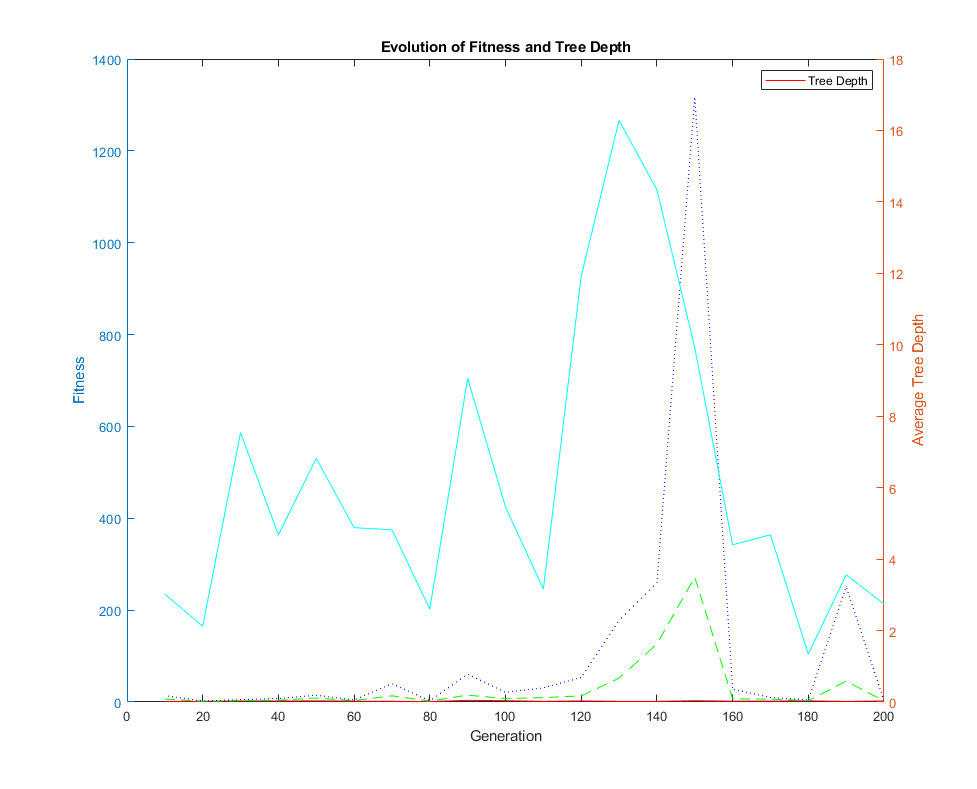
\includegraphics{evolution_of_fitness_vs_tree_depth.png}

}

\caption{\label{fig-plot}exanple plot with 200 generations}

\end{figure}%

The plot visualizes the evolutionary process of symbolic regression
using a genetic algorithm , highlighting the improvement in fitness
(error reduction) and changes in solution complexity (tree depth) across
generations. This approach aims to find mathematical expressions
(symbolic models) that best fit the training data
(A4\_trainingSamples.txt). Each line provides critical insights into the
algorithm's performance and the nature of solutions generated over time.

The \texttt{plotFigure} function visualizes the evolution of fitness and
tree depth over generations, aiding in the interpretation of the
algorithm's progress.

\begin{Shaded}
\begin{Highlighting}[]
\KeywordTok{function} \VariableTok{plotFigure}\NormalTok{(}\VariableTok{best\_fit}\OperatorTok{,} \VariableTok{avg\_fit}\OperatorTok{,} \VariableTok{worst\_fit}\OperatorTok{,} \VariableTok{tree\_depth}\OperatorTok{,} \VariableTok{gen}\NormalTok{)}
    \VariableTok{generations} \OperatorTok{=} \FloatTok{10}\OperatorTok{:}\FloatTok{10}\OperatorTok{:}\VariableTok{gen}\OperatorTok{;}
    \VariableTok{figure}\OperatorTok{;}
    \VariableTok{yyaxis} \VariableTok{left}
    \VariableTok{plot}\NormalTok{(}\VariableTok{generations}\OperatorTok{,} \VariableTok{best\_fit}\OperatorTok{,} \SpecialStringTok{\textquotesingle{}r\textquotesingle{}}\OperatorTok{,} \VariableTok{generations}\OperatorTok{,} \VariableTok{avg\_fit}\OperatorTok{,} \SpecialStringTok{\textquotesingle{}g\textquotesingle{}}\OperatorTok{,} \VariableTok{generations}\OperatorTok{,} \VariableTok{worst\_fit}\OperatorTok{,} \SpecialStringTok{\textquotesingle{}b\textquotesingle{}}\NormalTok{)}\OperatorTok{;}
    \VariableTok{xlabel}\NormalTok{(}\SpecialStringTok{\textquotesingle{}Generation\textquotesingle{}}\NormalTok{)}\OperatorTok{;}
    \VariableTok{ylabel}\NormalTok{(}\SpecialStringTok{\textquotesingle{}Fitness\textquotesingle{}}\NormalTok{)}\OperatorTok{;}
    \VariableTok{legend}\NormalTok{(}\SpecialStringTok{\textquotesingle{}Best\textquotesingle{}}\OperatorTok{,} \SpecialStringTok{\textquotesingle{}Average\textquotesingle{}}\OperatorTok{,} \SpecialStringTok{\textquotesingle{}Worst\textquotesingle{}}\NormalTok{)}\OperatorTok{;}
    
    \VariableTok{yyaxis} \VariableTok{right}
    \VariableTok{plot}\NormalTok{(}\VariableTok{generations}\OperatorTok{,} \VariableTok{tree\_depth}\OperatorTok{,} \SpecialStringTok{\textquotesingle{}c\textquotesingle{}}\NormalTok{)}\OperatorTok{;}
    \VariableTok{ylabel}\NormalTok{(}\SpecialStringTok{\textquotesingle{}Average Tree Depth\textquotesingle{}}\NormalTok{)}\OperatorTok{;}
    \VariableTok{legend}\NormalTok{(}\SpecialStringTok{\textquotesingle{}Tree Depth\textquotesingle{}}\NormalTok{)}\OperatorTok{;}
    
    \VariableTok{title}\NormalTok{(}\SpecialStringTok{\textquotesingle{}Evolution of Fitness and Tree Depth\textquotesingle{}}\NormalTok{)}\OperatorTok{;}
\KeywordTok{end}
\end{Highlighting}
\end{Shaded}

\textbf{Plot Explained:}

\emph{Fitness Evolution (Left Y-axis):}

Red Line (Best Fitness): Represents the fitness (error) of the best
individual in each generation. Green Line (Average Fitness): Shows the
average fitness (error) of the population in each generation. Blue Line
(Worst Fitness): Indicates the fitness (error) of the worst individual
in each generation. These lines show how the fitness (error) values
change over generations. The goal of the algorithm is typically to
minimize this fitness value, as it represents the error in predicting
the output (rf) based on the input (x, y).

\emph{Tree Depth Evolution (Right Y-axis):}

Cyan Line (Average Tree Depth): Displays the average depth of the trees
in the population for each generation. The depth of the trees is an
indicator of their complexity. Genetic programming often evolves trees
of varying depths, and monitoring the average tree depth helps in
understanding the complexity of the solutions found over generations.

\emph{X-axis (Generation):}

Each point on the x-axis represents a specific generation number
(10:10:gen), where gen is the total number of generations specified in
the code. Interpretation: Fitness Lines (Red, Green, Blue): Ideally, you
want to see the red (best fitness) line decreasing over generations,
indicating improvement in the best solution found. The green (average
fitness) and blue (worst fitness) lines provide context on the overall
performance of the population.

\emph{Tree Depth Line (Cyan):} Monitoring the tree depth helps in
understanding if the algorithm is converging towards simpler or more
complex solutions. An increase in average tree depth might indicate
overfitting or increasing complexity of solutions.

\textbf{Specific Colors in the Plot:} Green Line: Represents the average
fitness (error) of the population. Blue Line: Represents the worst
fitness (error) in the population. Cyan Line: Represents the average
depth of trees in the population. These lines collectively show how the
genetic algorithm progresses in terms of fitness (error minimization)
and the complexity of the evolved solutions (average tree depth).

The plot helps in understanding how the fitness of the population
improves over time and how the complexity of the solutions (tree depth)
changes.

\subsection{Conclusion}\label{conclusion}

The MATLAB implementation of genetic programming

for symbolic regression is a robust approach that leverages the power of
evolutionary algorithms to discover optimal mathematical expressions.
Key features include structured functions, effective randomization,
detailed logging, and clear visualization. This review highlights the
importance of genetic diversity, modular programming, and the use of
tree structures for representing mathematical expressions. These
elements collectively enhance the effectiveness of symbolic regression
using genetic algorithms.

\subsubsection{References}\label{references}

this part is still uderconstruction to be continued later



\end{document}
